\documentclass{TDP003mall}



\newcommand{\version}{Version 0.1}
\author{Nils Bark, \url{nilba048@student.liu.se}\\
  Hadi Ansari, \url{hadan326@student.liu.se}}
\title{Dokumentmall}
\date{2020-11-27}
\rhead{Nils Bark\\
Hadi Ansari}



\begin{document}
\projectpage
\section{Revisionshistorik}
\begin{table}[!h]
\begin{tabularx}{\linewidth}{|l|X|l|}
\hline
Ver. & Revisionsbeskrivning & Datum \\\hline
0.1 & Första utkast skapat & 2020-11-27\\\hline
\end{tabularx}
\end{table}

\section{Beskrivning av Game\_Object}
\texttt{Game\_Object} är en \texttt{abstract struct} som alla klasser i spelet ärver ifrån. 
\texttt{Game\_Object} låter oss därmed uppdatera alla andra object i spelet. 
Detta sker via funktionen \texttt{tick()} som tar in en parameter av typen \texttt{sf::Time} och uppdaterar med hjälp av den positionen för alla objekt på skärmen.
\texttt{Tick()} är en \texttt{virtual} funktion som kan överskridas i de härledda klasserna.
Tack vare tidsberäkningen är vi oberoende av spelets bildfrekvens och tiden det tar att hantera alla händelser i loopen.
Datamedlemmarna i basklassen kommer att initieras av de härledda klassernas struktur, 
till exempel kommer spelarens \texttt{speed} att initieras när spelaren skapas och inte innan.

\begin{itemize}
\item \texttt{Center} är en variabel av typen \texttt{Vector2f} som sparar en figurs origo.
\item \texttt{Speed} är en variabel av typen \texttt{float} som används för att bestämma objekts hastighet. 
\item \texttt{Sprite} är en variabel av typen \texttt{sf::Sprite}. Den fungerar som figurens kropp och kan täckas av en textur.
\texttt{sprite} används även för att kontrollera kollision med andra objekt.
\item \texttt{Texture} är en variabel som tar in en bild och använder den som textur för ett objekt.
\end{itemize}

\section{Beskrivning av Player}
\texttt{Player} representerar det objekt som användaren kommer att ha kontroll över under spelets gång. 
Det är en härledd klass av \texttt{Game\_Object} och ärver därmed alla datamedlemmar och funktioner därifrån. 
Den har också en aggregations-relation till \texttt{Bullet} och \texttt{Power-ups} härledda klasser.
Den har en funktion \texttt{process\_event()} som läser in nedtryckta tangenter via \texttt{sf::Keyboard::Key} 
och använder sig av den informationen för att antingen kalla på \texttt{shoot()} eller uppdatera spelarens \texttt{location}. 
Den överskrider \texttt{tick()} för att kunna läsa in en ny \texttt{location} som \texttt{process\_event} har uppdaterat och sätta spelarens position baserat på det.
Förutom de variabler den ärver har \texttt{Player} även en \texttt{int health} som avgör spelarens liv. 
I spelarens konstruktor initieras spelarens liv (till 3), \texttt{location} och \texttt{speed}.
Här tar även \texttt{texture} och importerar den bild som ska representera spelaren och täcker \texttt{sprite} med den.

För att skjuta mot de fiender spelaren kommer stöta på använder sig \texttt{Player} av funktionen \texttt{shoot()}. 
Den kallas på när \texttt{process\_event} läser ett nedtryckt mellanslag och skapar då ett bullet-objekt 
som färdas rakt åt höger med konstant hastighet. Vid kollision med fiender ska det skada dem, 
annars förstör objektet då det hamnar utanför spelplanen.

Det ska finnas en kollisionshanterande funktion i klassen som med hjälp av spelarens \texttt{location} kontrollerar om den har kolliderat med något annat object 
och utför då korrekt respons till kollisionen (eller ignorerar kollisionen ifall ingen respons krävs). 
\section{Diskussion}
Så pass tidigt i projektet finns inte mycket nyanserad diskussion att ha kring för- och nackdelar av det lilla som har gjorts hittills. 
Dock är en fördel att alla objekt i spelet fördelas olika klasser som har korrekt relationer till varandra, vilket leder till att spelet hänger ihop på ett bra sätt.

\section{Externa filformat} 
Planen är att banor ska läsas in från externa filer, så som JSON eller txt. Om bör-kravet att implementera topplistor över poäng uppnås så är planen att spara poängen i en JSON fil.
\begin{figure}[h!]
\centering
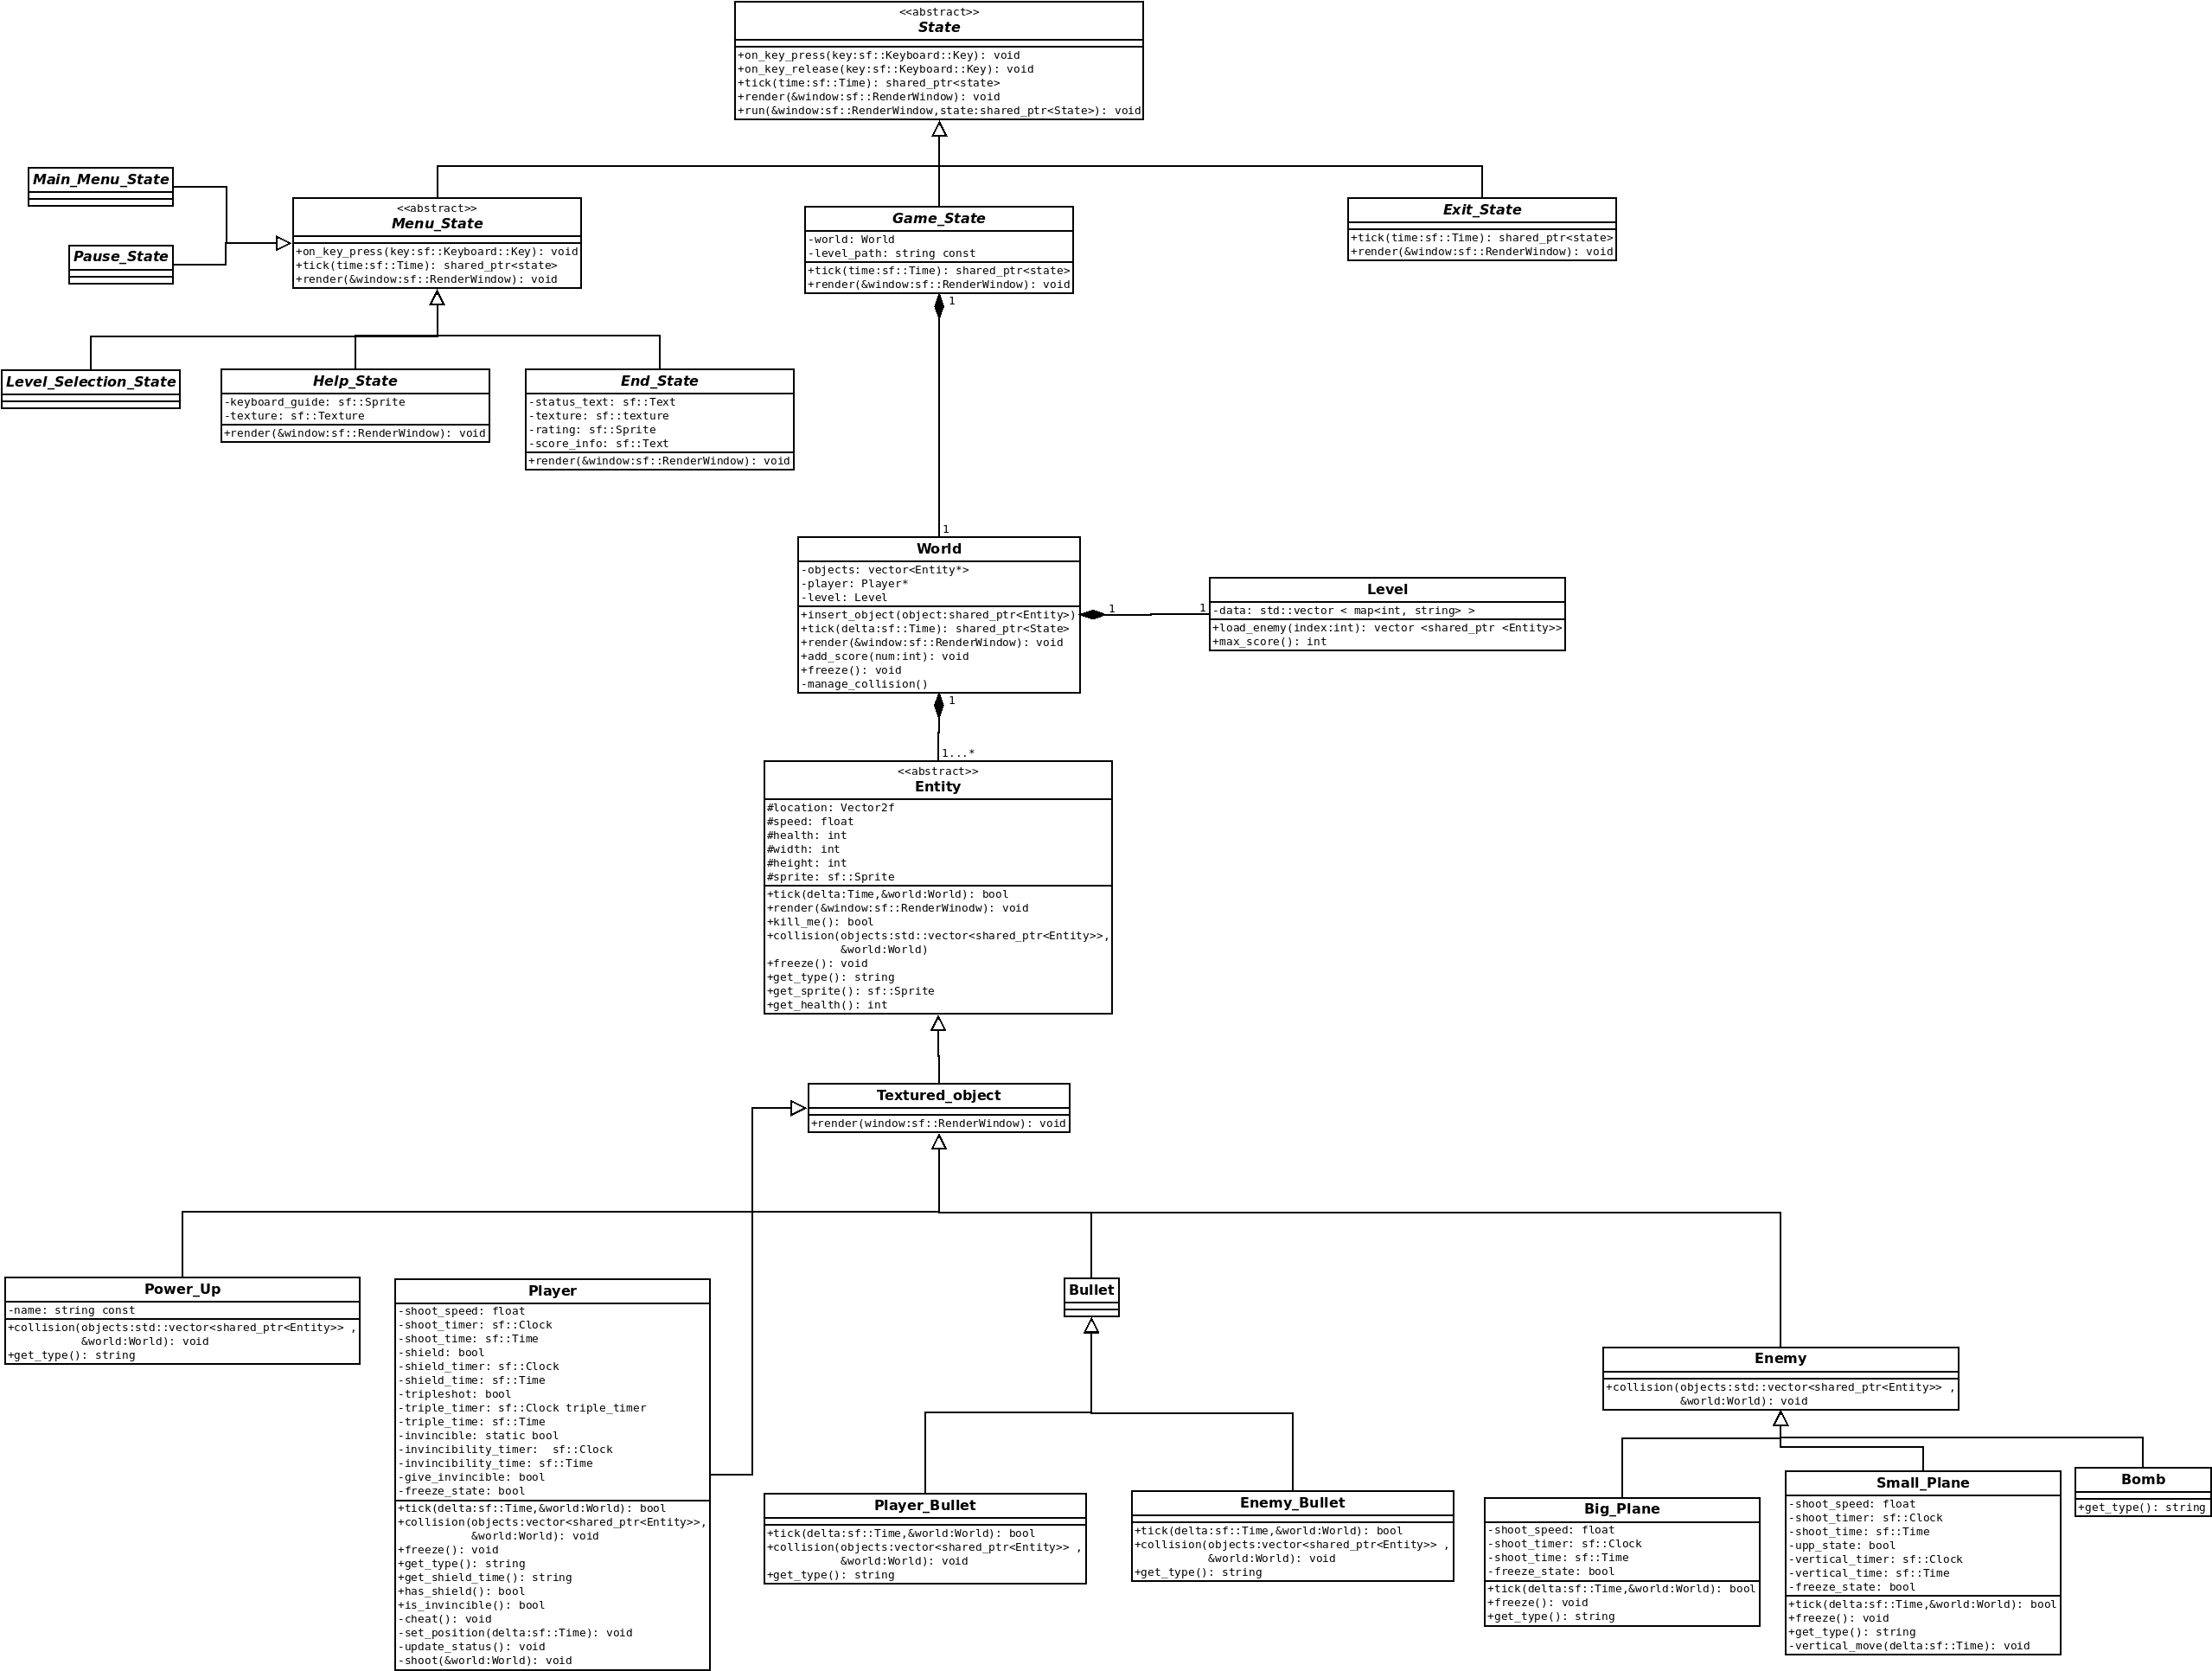
\includegraphics[scale=0.5]{UML_diagram.png}
\label{}
\caption{UML-diagram över spelet}
\end{figure}
\end{document}
